\iffalse
\documentclass[journal,10pt,twocolumn]{article}
\usepackage{graphicx}
\usepackage[margin=0.5in]{geometry}
\usepackage[cmex10]{amsmath}
\usepackage{amssymb}
\usepackage{array}
\usepackage{booktabs}
\usepackage{mathtools}
\usepackage{dirtree}
\usepackage{xcolor}
\usepackage{float}
\usepackage[justification=centering,font={rm,md,scriptsize}]{caption}
\usepackage{enumitem}
\usepackage{listings}
\usepackage{mathtools}
\usepackage{fancyvrb}
\usepackage{hyperref}

%Add chapter functionality in IEEEtran class
\newcounter{Chapcounter}
\newcommand\showmycounter{\addtocounter{Chapcounter}{1}\themycounter}
\newcommand{\chapter}[1] 
{ {\centering          
  \addtocounter{Chapcounter}{1} \large \textbf{Chapter \theChapcounter ~#1}}  
  \addcontentsline{toc}{section}{Chapter ~\theChapcounter~~ #1}    
  \setcounter{section}{0}
}
%%%%

\counterwithin{enumi}{section}
\counterwithin{equation}{enumi}
\counterwithin{figure}{enumi}

\renewcommand\thesection{\theChapcounter.\arabic{section}}
%\renewcommand\thesectiondis{\theChapcounter.\arabic{section}}
\newcommand\figref{Fig.~\ref}

\setenumerate{label=\thesection.\arabic*}

\lstset{
  basicstyle=\ttfamily,
  columns=fullflexible,
  frame=single,
  breaklines=true,
  postbreak=\mbox{\textcolor{red}{$\hookrightarrow$}\space},
}

\providecommand{\mbf}{\mathbf}
\providecommand{\pr}[1]{\ensuremath{\Pr\left(#1\right)}}
\providecommand{\qfunc}[1]{\ensuremath{Q\left(#1\right)}}
\providecommand{\sbrak}[1]{\ensuremath{{}\left[#1\right]}}
\providecommand{\lsbrak}[1]{\ensuremath{{}\left[#1\right.}}
\providecommand{\rsbrak}[1]{\ensuremath{{}\left.#1\right]}}
\providecommand{\brak}[1]{\ensuremath{\left(#1\right)}}
\providecommand{\lbrak}[1]{\ensuremath{\left(#1\right.}}
\providecommand{\rbrak}[1]{\ensuremath{\left.#1\right)}}
\providecommand{\cbrak}[1]{\ensuremath{\left\{#1\right\}}}
\providecommand{\lcbrak}[1]{\ensuremath{\left\{#1\right.}}
\providecommand{\rcbrak}[1]{\ensuremath{\left.#1\right\}}}
\newcommand{\sgn}{\mathop{\mathrm{sgn}}}
\providecommand{\abs}[1]{\left\vert#1\right\vert}
\providecommand{\res}[1]{\Res\displaylimits_{#1}} 
\providecommand{\norm}[1]{\left\lVert#1\right\rVert}
\providecommand{\mtx}[1]{\mathbf{#1}}
\providecommand{\mean}[1]{E\left[ #1 \right]}
\providecommand{\fourier}{\overset{\mathcal{F}}{ \rightleftharpoons}}
\providecommand{\ztrans}{\overset{\mathcal{Z}}{ \rightleftharpoons}}
\providecommand{\system}{\overset{\mathcal{H}}{ \longleftrightarrow}}
\newcommand{\solution}{\noindent \textbf{Solution: }}
\newcommand{\cosec}{\,\text{cosec}\,}
\providecommand{\dec}[2]{\ensuremath{\overset{#1}{\underset{#2}{\gtrless}}}}
\newcommand{\myvec}[1]{\ensuremath{\begin{pmatrix}#1\end{pmatrix}}}
\newcommand{\mydet}[1]{\ensuremath{\begin{vmatrix}#1\end{vmatrix}}}
\providecommand{\gauss}[2]{\mathcal{N}\ensuremath{\left(#1,#2\right)}}
\newcommand*{\permcomb}[4][0mu]{{{}^{#3}\mkern#1#2_{#4}}}
\newcommand*{\perm}[1][-3mu]{\permcomb[#1]{P}}
\newcommand*{\comb}[1][-1mu]{\permcomb[#1]{C}}

\let\vec\mathbf

\def\putbox#1#2#3{\makebox[0in][l]{\makebox[#1][l]{}\raisebox{\baselineskip}[0in][0in]{\raisebox{#2}[0in][0in]{#3}}}}
     \def\rightbox#1{\makebox[0in][r]{#1}}
     \def\centbox#1{\makebox[0in]{#1}}
     \def\topbox#1{\raisebox{-\baselineskip}[0in][0in]{#1}}
     \def\midbox#1{\raisebox{-0.5\baselineskip}[0in][0in]{#1}}

\begin{document}

\title{Random Numbers}
\author{Sampath Govardhan}

\maketitle

\tableofcontents

\bigskip

\fi

\section{Uniform Random Numbers}
Let $U$ be a uniform random variable between 0 and 1.
\begin{enumerate}
\item Generate $10^6$ samples of $U$ using a C program and save into a file called uni.dat .
\label{prob:uni_gen}
\\
\solution Download the following files and execute the  C program.
\begin{lstlisting}
codes/include/coeffs.h
codes/src/uni_gen_stat.c
\end{lstlisting}

%
\item
Load the uni.dat file into python and plot the empirical CDF of $U$ using the samples in uni.dat. The CDF is defined as
\begin{align}
F_{U}(x) = \pr{U \le x}
\end{align}
\\
\solution  The following code plots \figref{fig:uni_cdf}
\begin{lstlisting}
codes/src/2.1.py
\end{lstlisting}
\begin{figure}[h]
\centering
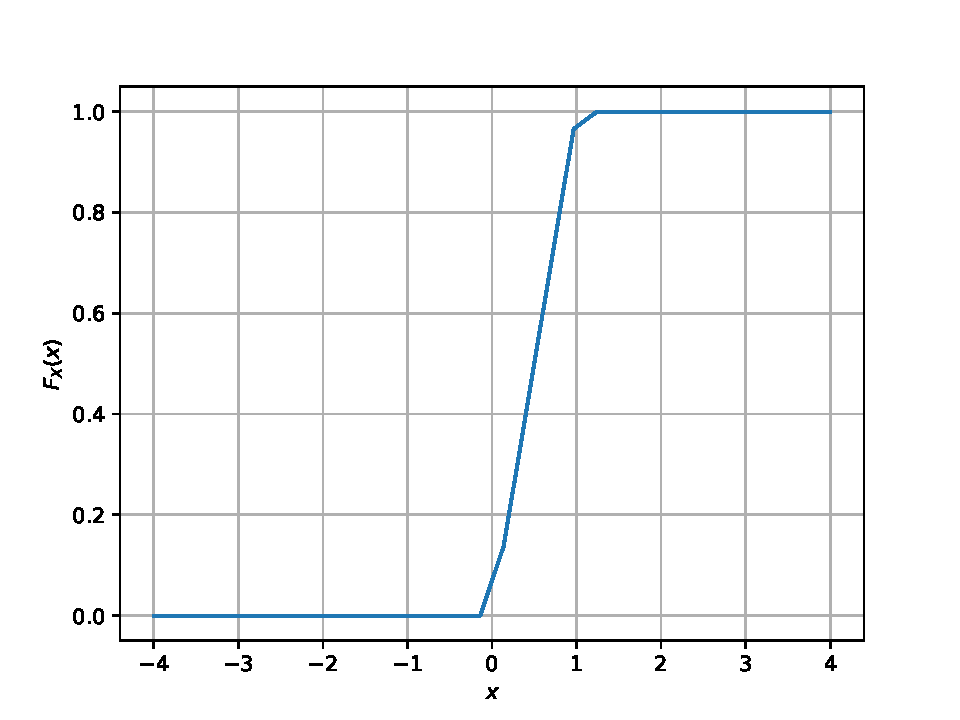
\includegraphics[width=\columnwidth]{./chapters/ch2/figs/uni_cdf.pdf}
\caption{The CDF of $U$}
\label{fig:uni_cdf}
\end{figure}

%
\item
Find a  theoretical expression for $F_{U}(x)$.\\
\solution
\begin{align} 
F_{U}(x) = \int_{-\infty}^{x} f_{U}(x)\,dx
\label{eq:pdf_to_cdf}
\end{align}
For the uniform random variable $U$, $f_{U}(x)$ is given by  
\begin{align}
	f_U(x) &= 
	\begin{cases}
	1 &  0 \le x \le  1
	\\
	0 & elsewhere
	\\
	\end{cases}
	\label{eq:uni_pdf}
\end{align}
Substituting \eqref{eq:uni_pdf} in \eqref{eq:pdf_to_cdf}, $F_U(x)$ is found to be
\begin{align}
	F_U(x) &= 
	\begin{cases}
	0 & x < 0
	\\	
	x & 0 \le x \le  1
	\\
	1 & x > 0
	\\
	\end{cases}
	\label{eq:uni_cdf}
\end{align}

\item
\label{prob:print_uni}
The mean of $U$ is defined as
%
\begin{equation}
E\sbrak{U} = \frac{1}{N}\sum_{i=1}^{N}U_i
\end{equation}
%
and its variance as
%
\begin{equation}
\text{var}\sbrak{U} = E\sbrak{U- E\sbrak{U}}^2 
\end{equation}

Write a C program to  find the mean and variance of $U$.\\
\solution The following code prints the mean and variance of $U$
\begin{lstlisting}
codes/src/uni_gen_stat.c
\end{lstlisting}

\item Verify your result theoretically given that
%
\begin{equation}
E\sbrak{U^k} = \int_{-\infty}^{\infty}x^kdF_{U}(x)
\end{equation}\\
\solution For a random variable $X$, the mean $\mu_X$ and variance $\sigma_X^2$ are given by
\begin{align}
	\label{eq:mean_exp}
	\mu_X &= E\sbrak{X} = \int_{-\infty}^{\infty}xdF_{U}(x) \\
	\label{eq:var_exp}
	\sigma_X^2 &= E\sbrak{X^2} - \mu_X^2 = \int_{-\infty}^{\infty}x^2dF_{U}(x) - \mu_X^2
\end{align}  
Substituting the CDF of $U$ from \eqref{eq:uni_cdf} in \eqref{eq:mean_exp} and \eqref{eq:var_exp}, we get
\begin{align}
	\label{eq:mean_uni}
	\mu_U &= \frac{1}{2} \\
	\label{eq:var_uni}
	\sigma_U^2 &= \frac{1}{12}
\end{align}  
which match with the values printed in problem \ref{prob:print_uni}
\end{enumerate}
\section{Central Limit Theorem}
\begin{enumerate}
%
%
\item
Generate $10^6$ samples of the random variable
%
\begin{equation}
X = \sum_{i=1}^{12}U_i -6
\end{equation}
%
using a C program, where $U_i, i = 1,2,\dots, 12$ are  a set of independent uniform random variables between 0 and 1
and save in a file called gau.dat\\
\solution Download the following files and execute the  C program.
\begin{lstlisting}
codes/include/coeffs.h
codes/src/gau_gen_stat.c
\end{lstlisting}
%
\item
Load gau.dat in python and plot the empirical CDF of $X$ using the samples in gau.dat. What properties does a CDF have?
\\
\solution The CDF of $X$ is plotted in \figref{fig:gauss_cdf}
\begin{figure}[H]
\centering
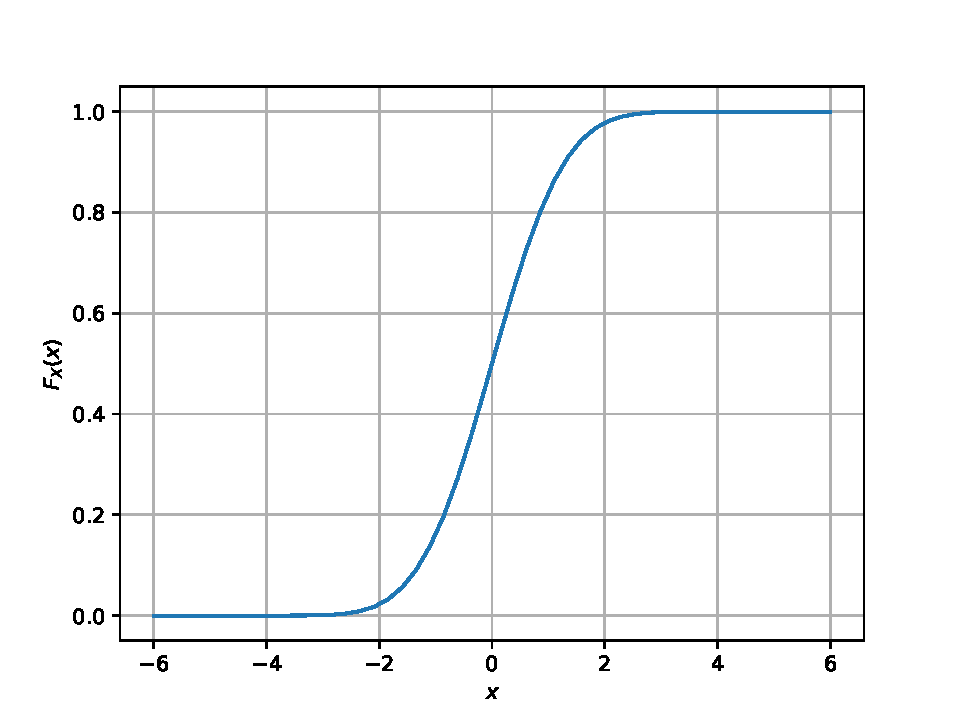
\includegraphics[width=\columnwidth]{./chapters/ch2/figs/gau_cdf.pdf}
\caption{The CDF of $X$}
\label{fig:gauss_cdf}
\end{figure}
The properties of a CDF are
\begin{eqnarray}
	F_X(-\infty) = 0\\
	F_X(\infty) = 1\\
	\frac{dF_X(x)}{dx} \ge 0
\end{eqnarray}
\item
Load gau.dat in python and plot the empirical PDF of $X$ using the samples in gau.dat. The PDF of $X$ is defined as
\begin{align}
p_{X}(x) = \frac{d}{dx}F_{X}(x)
\label{eq:cdf_to_pdf}
\end{align}
What properties does the PDF have?
\\
\solution The PDF of $X$ is plotted in \figref{fig:gauss_pdf} using the code below
\begin{lstlisting}
codes/src/2.2.py
\end{lstlisting}

\begin{figure}[h]
\centering
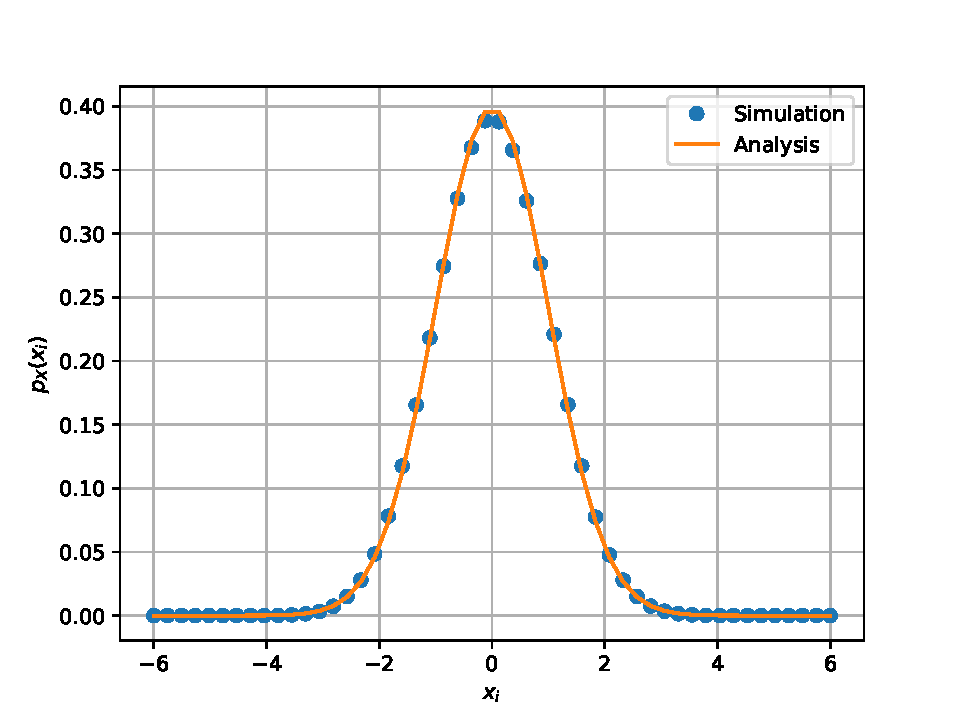
\includegraphics[width=\columnwidth]{./chapters/ch2/figs/gau_pdf.pdf}
\caption{The PDF of $X$}
\label{fig:gauss_pdf}
\end{figure}

The properties of PDF are
\begin{eqnarray}
	f_X(x) \ge 0\\
	\int_{-\infty}^{\infty} f_X(x) \,dx = 1
\end{eqnarray}

\item Find the mean and variance of $X$ by writing a C program.
\solution The following code prints the mean and variance of $X$
\begin{lstlisting}
codes/src/gau_gen_stat.c
\end{lstlisting}

\item Given that 
\begin{align}
p_{X}(x) = \frac{1}{\sqrt{2\pi}}\exp\brak{-\frac{x^2}{2}}, -\infty < x < \infty,
\label{eq:gau_pdf}
\end{align}
repeat the above exercise theoretically.\\
\solution Substituting the PDF from \eqref{eq:gau_pdf} in \eqref{eq:mean_exp},
\begin{flalign}
	\mu_X &= \int_{-\infty}^{\infty} \frac{x}{\sqrt{2\pi}}\exp\brak{-\frac{x^2}{2}} \,dx&\\
	\intertext{Using}&\\
	\int x \cdot \exp \left( -a x^2 \right) \mathrm{d}x &= -\frac{1}{2a} \cdot \exp \left( -a x^2 \right)&\\
	\mu_X &= \frac{1}{\sqrt{2\pi}}\left[-\exp\brak{-\frac{x^2}{2}}\right]_{-\infty}^{\infty}&\\  
	\mu_X &= 0
\end{flalign}
Substituting $\mu_X$ and the PDF in \eqref{eq:var_exp} to compute variance,
\begin{flalign}
	\sigma_X^2 &= \int_{-\infty}^{\infty} \frac{x^2}{\sqrt{2\pi}}\exp\brak{-\frac{x^2}{2}} \,dx&\\ \nonumber
	\intertext{Substituting} t &= \frac{x^2}{2},&\\	
	\sigma_X^2 &= \frac{2}{\sqrt{\pi}} \int_{0}^{\infty} t^{\frac{1}{2}}\exp\brak{-t} \,dt&\\	\nonumber
	&= \frac{2}{\sqrt{\pi}} \int_{0}^{\infty} t^{\frac{3}{2}-1}\exp\brak{-t} \,dt&\\
	\intertext{Using the gamma function} \Gamma(x) &= \int_{0}^{\infty} z^{x-1} \cdot e^{-z} \, \mathrm{d}z \,&\\
	\sigma_X^2 &= \frac{2}{\sqrt{\pi}}\Gamma(\frac{3}{2})&\\	\nonumber
	&= \frac{2}{\sqrt{\pi}}\frac{\sqrt{\pi}}{2}&\\	\nonumber
	&=1	
\end{flalign}
%
\end{enumerate}
\section{From Uniform to Other}
\begin{enumerate}
%
\item
Generate samples of 
%
\begin{equation}
V = -2\ln\brak{1-U}
\end{equation}
%
and plot its CDF. \\
\solution The samples for $U$ are loaded from uni.dat file generated in problem \ref{prob:print_uni}. The CDF of $V$ is plotted in \figref{fig:log_uni_cdf} using the code below, 
\begin{lstlisting}
codes/src/2.3.py
\end{lstlisting}
\begin{figure}[H]
\centering
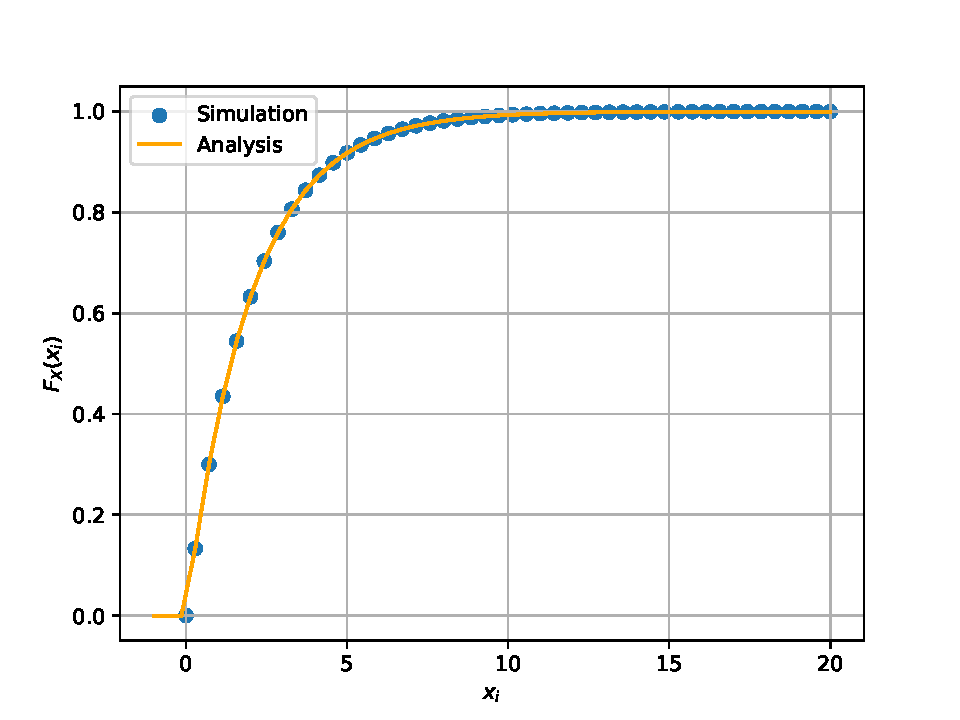
\includegraphics[width=\columnwidth]{./chapters/ch2/figs/log_uni_cdf.pdf}
\caption{The CDF of $V$}
\label{fig:log_uni_cdf}
\end{figure}
\item Find a theoretical expression for $F_V(x)$.
\begin{flalign}
	F_V(x) &= P(V < x)&\\
	&= P(-2\ln\brak{1-U} < x)&\\
	&= P(U < 1 - e^{\frac{-x}{2}})&\\
	&= F_U(1 - e^{\frac{-x}{2}})
\end{flalign}
Using $F_U(x)$ defined in \eqref{eq:uni_cdf},
\begin{align}
	F_V(x) &=
	\begin{cases}
		0 & x < 0\\
		1 - e^{\frac{-x}{2}} & x \ge 0
	\end{cases}
\end{align} 
%
%\item
%Generate the Rayleigh distribution from Uniform. Verify your result through graphical plots.
\end{enumerate}

\section{Triangular Distribution}
%
\begin{enumerate}
\item Generate 
	\begin{align}
		T = U_1+U_2
	\end{align}\\
\solution Download the following files and execute the  C program.
\begin{lstlisting}
codes/include/coeffs.h
codes/src/two_uni_gen.c
\end{lstlisting}
\item Find the CDF of $T$.\\
\solution Loading the samples from uni1.dat and uni2.dat in python, the CDF is plotted in \figref{fig:tri_cdf} 
\begin{figure}[h]
\centering
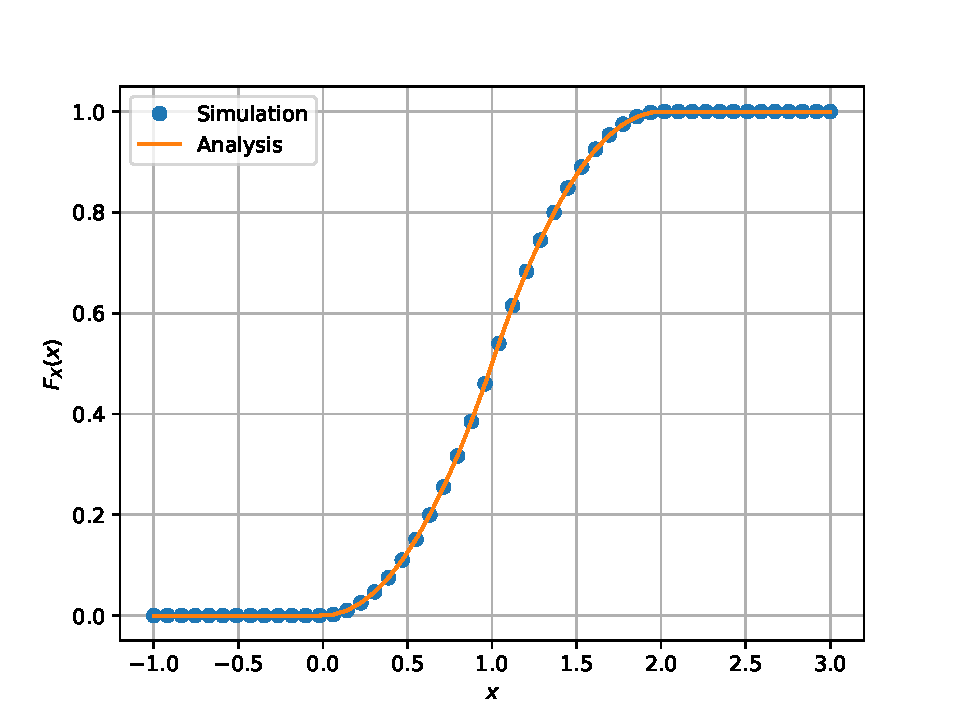
\includegraphics[width=\columnwidth]{./chapters/ch2/figs/tri_cdf.pdf}
\caption{The CDF of $T$}
\label{fig:tri_cdf}
\end{figure}
\item Find the PDF of $T$.\\
\solution The PDF of $T$ is plotted in \figref{fig:tri_pdf} using the code below
\begin{lstlisting}
codes/src/2.4.py
\end{lstlisting}
\begin{figure}[h]
\centering
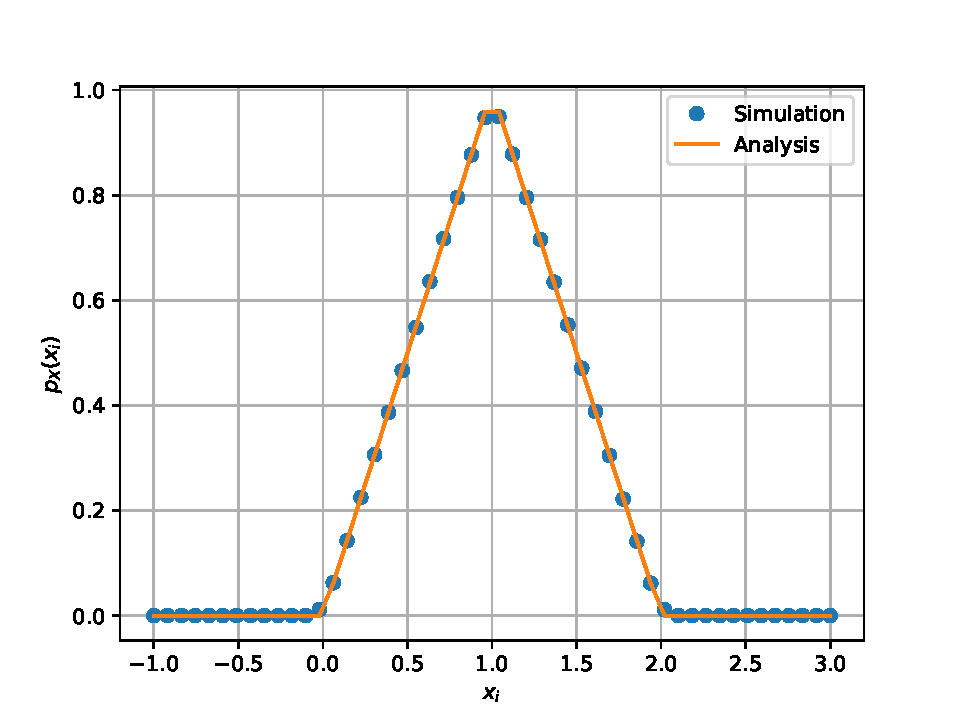
\includegraphics[width=\columnwidth]{./chapters/ch2/figs/tri_pdf.pdf}
\caption{The PDF of $T$}
\label{fig:tri_pdf}
\end{figure}
\item Find the theoretical expressions for the PDF and CDF of $T$.\\
\solution Since $T$ is the sum of two independant random variables $U1$ and $U2$, the PDF of $T$ is given by
\begin{flalign}
	p_T(x) &= p_{U1}(x) \ast p_{U2}(x)
\end{flalign}
Using the PDF of $U$ from \eqref{eq:uni_pdf}, the convolution results in
\begin{align}
	p_T(x) &=
	\begin{cases}
		0 & x < 0\\
		x & 0 \le x \le 1\\
		2-x & 1 \le x \le 2\\
		0 & x > 2
	\end{cases}
	\label{eq:tri_pdf}
\end{align}
The CDF of $T$ is found using \eqref{eq:pdf_to_cdf} by replacing $U$ with $T$. Evaluating the integral for the piecewise function $p_T(x)$, 
\begin{align}
	F_T(x) &=
	\begin{cases}
		0 & x < 0\\
		\frac{x^2}{2} & 0 \le x \le 1\\
		2x-\frac{x^2}{2}-1 & 1 \le x \le 2\\
		1 & x > 2
	\end{cases}
\end{align}
\item Verify your results through a plot. \\
\solution The theoretical and numerical plots for the CDF and PDF of $T$ closely match in \figref{fig:tri_cdf} and \figref{fig:tri_pdf}
\end{enumerate}



%\end{document}
